\documentclass{beamer}
\usepackage{amsmath, amssymb}
\usepackage{bm}
\usepackage{luatexja}
\usepackage{mathrsfs}              % 花文字
\usepackage{multirow}              % 表結合
\usepackage{float}                 % 図の位置制御
\usepackage{url}                   % URL表示
\usepackage{type1cm}               % フォント調整
\usepackage{here}                  % H位置指定
\usepackage{physics}               % 量子力学向け記法
\usepackage{graphicx}
% \usepackage{unicode-math}
% \setmathfont{Latin Modern Math} % or STIX Two Math, XITS Math, etc.
% ページ番号を右下に表示
\setbeamertemplate{footline}{
  \leavevmode%
  \hbox{%
    \begin{beamercolorbox}[wd=.95\paperwidth,ht=2.5ex,dp=1ex,left]{author in head/foot}%
      \hfill%
      \usebeamerfont{page number in head/foot}\insertframenumber{} / \inserttotalframenumber
      \hspace*{2ex}
    \end{beamercolorbox}%
  }%
}
\setbeamertemplate{navigation symbols}{}  % ナビゲーションアイコン非表示

\title{量子閉じ込め場内の電子状態\\\small ~ 実空間差分法に基づく数値計算 ~}
\author{早稲田大学 先進理工学研究科 電気・情報生命専攻 武田研究室\\新井開智・平田慧仁郎・藤原大地}
\date{\today}
\begin{document}

\frame{\titlepage}

\begin{frame}{目次}
\begin{enumerate}
  \item 本演習の目的
  \item 対象系
  \item ハミルトニアンの構築
  \item 数値計算
  \item 計算結果の解析と物理的解釈
\end{enumerate}
\end{frame}

\begin{frame}{1. 本演習の目的}
量子閉じ込め場内の電子はエネルギー準位が離散化される.\\
  この演習では,\textbf{半導体量子ドット中の電子状態}を,解析的および数値的手法を用いて解明することを目的とする.

\end{frame}



\begin{frame}{2. 対象系}
今回の演習では,InSb材料によって形成された$100nm$サイズの二次元円形量子ドットを対象に,その中に閉じ込められた電子状態を解析する.
\begin{center}
  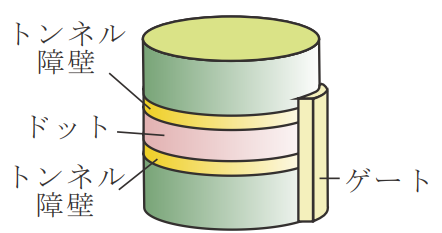
\includegraphics[width=0.5\linewidth]{images/ドット.png} \\
  図2.1:InSb 量子ドット構造 \\
  \vspace{0.5em}
  {\tiny 勝本信吾 著「半導体物理学」より引用}
\end{center}


量子ドットとは,電子の量子力学的な性質(粒子性と波動性)を顕著に引き出す\textbf{人工的な原子様構造}であり,次の二つの特長がある.
\begin{itemize}
  \item \textbf{電子数を1個単位で制御できる}:  \\
  \item \textbf{波動性が顕著になるサイズ(10〜100 nm)}:  \\
  \rightarrow 閉じ込めに応じて,エネルギー準位が離散化される.
\end{itemize}



% \begin{flushright}
% 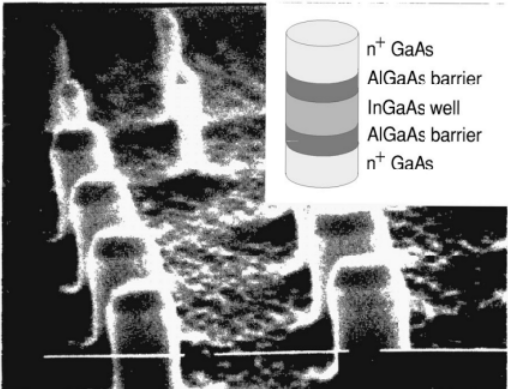
\includegraphics[width=0.3\linewidth]{images/量子ドット.png}\\
% 図1:量子ドット
% \end{flushright}

\end{frame}

% ...(ここに続く仮定・解析・差分法・行列化・結果解析・課題を順に展開)

\begin{frame}{3. ハミルトニアンの構築}

  電子状態の解析にはシュレディンガー方程式を解く必要がある.
  \begin{equation}
    \hat{\mathcal{H} } \psi = E \psi
  \end{equation}  
  
  この演習では対象系のハミルトニアンを以下の二つの仮定を用いて構築する.
  \begin{itemize}
    \item \textbf{有効質量近似}  \\
    \rightarrow 結晶中の電子のふるまいを,有効質量と有効誘電率を使って“真空中の電子”になぞらえる近似
    \item \textbf{ハイブリッドポテンシャル}  \\
    \rightarrow 量子ドットの有効ポテンシャルを調和振動子と円筒壁という二成分を組み合わせたポテンシャル(\textbf{ハイブリッドポテンシャル})とモデル化
  \end{itemize}
\end{frame}
  
\begin{frame}{3.1 有効質量近似}
  半導体中の電子に対して\textbf{有効質量近似}を導入する.
  これは結晶が作る周期的ポテンシャルの効果を電子の有効質量に押し込める近似である.
  InSbの有効質量 $m^*=m_rm_o$ を用いて以下のように式を立てる:

  \begin{equation}
    \left[ -\frac{\hbar^2}{2 m^*} \nabla^2 + V \right] \psi = E \psi
  \end{equation}
  

\end{frame}  

\begin{frame}{3.2 ハイブリッドポテンシャル}
\footnotesize
  量子ドットのポテンシャルは,一様電荷分布のポアソン方程式解から\textbf{調和振動子型のポテンシャル}に近い形状をとると考えられる.
  
  \vspace{-1.0em}
  \begin{minipage}{0.7\textwidth}
  \begin{equation}
  V_{調和}(r)=\frac{1}{2}m\omega^2r^2
  \end{equation}
  \end{minipage}
  \hfill
  \vspace{-1.0em}
  \begin{minipage}{0.28\textwidth}
  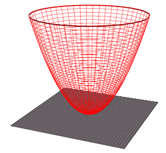
\includegraphics[width=0.8\linewidth]{images/調和.png} \\
  \end{minipage}
  一方,量子ドットの有限性から,\textbf{円筒の無限に高い障壁}を仮定する.
  \begin{minipage}{0.7\textwidth}
  \begin{equation}
  V_{円筒}(r) =
  \begin{cases}
  0 & (r < R) \\
  \infty & (r \geq R)
  \end{cases}
  \end{equation}
  \end{minipage}
  \hfill
    \vspace{-1.0em}
  \begin{minipage}{0.28\textwidth}
  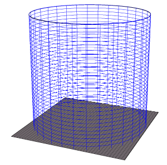
\includegraphics[width=0.8\linewidth]{images/円筒.png} \\
  \end{minipage}
  
  本演習では,こうした構造的特徴を踏まえ,\textbf{中心部で調和型,外縁で円筒壁型}\\
  となる\textbf{ハイブリッドポテンシャル}を用意した.
    \vspace{-1.0em}
  \begin{minipage}{0.7\textwidth}
  \begin{equation}
  V_{ハイブリッド}(r) =
  \begin{cases}
  V_{調和}(r) & (r < R) \\
  V_{円筒}(r) & (r \geq R)
  \end{cases}
  \end{equation}
  \end{minipage}
  \hfill
  \begin{minipage}{0.28\textwidth}
  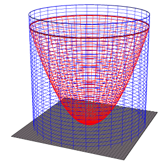
\includegraphics[width=0.8\linewidth]{images/ハイブリッド.png} \\
  \end{minipage}
  
  \end{frame}
  % 図3.1:量子ドットのポテンシャル
  % \begin{center}
  % 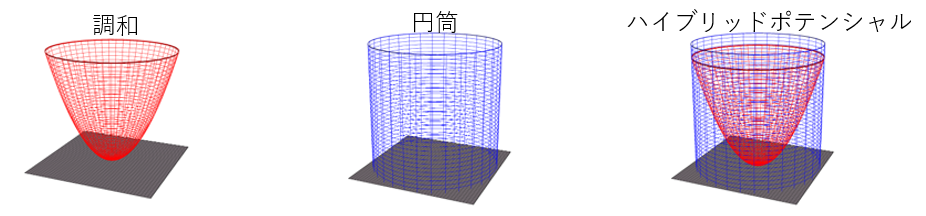
\includegraphics[width=0.5\linewidth]{images/三種盛り.png} \\
  % 図3.1:量子ドットのポテンシャル
  % \end{center}

\begin{frame}{4.数値計算}

今回の数値計算では次の二つのテクニックを組み合わせた.

\begin{itemize}
  \item \textbf{有効原子単位系}:  \\
  \rightarrow 数式を簡潔にし,数値計算の精度を向上させる単位系を導入する
  \item \textbf{実空間差分法}:  \\
  \rightarrow 空間座標を差分化して,偏微分方程式を連立方程式に置き換える
\end{itemize}
\end{frame}
  \begin{frame}{4.1 有効原子単位系}
    \textbf{原子単位系}は,基本定数(電子の電荷 $e$,電子質量 $m_e$,プランク定数 $\hbar$,クーロン定数 $1/4\pi\varepsilon_0$)を全て単位1とする.
    \textbf{有効原子単位系}は,\textbf{有効質量近似}による影響を単位系に押し込めたものである.

    \begin{center}
    {\tiny
    \begin{tabular}{|c|c|c|c|}
    \hline
    \textbf{物理量} & \textbf{SI単位系} & \textbf{原子単位系} & \textbf{有効原子単位系} \\
    \hline
    電荷 & $C$ & 電気素量: $e$ & $e$ \\
    \hline
    質量 & $kg$ & 電子質量: $m_e$ & $m^* = m_r m_0$ \\
    \hline
    角運動量 & $J\cdot s$ & プランク定数: $\hbar$ & $\hbar$ \\
    \hline
    長さ & $m$ & ボーア半径: $a_0$ & $a_0^* = \frac{\varepsilon_r}{m_r} a_0$ \\
    \hline
    エネルギー & $J$ & $E_h$ & $E_h^* = \frac{m_r}{\varepsilon_r^2} E_h$ \\
    \hline
    \end{tabular}
    }
    \end{center}
    
    


    有効原子単位系での\textbf{シュレディンガー方程式}が簡略化される.

      {\Large
      \begin{equation}
      \displaystyle
      \left[ -\frac{1}{2} \nabla^2 + V \right] \phi = E \phi
      \end{equation}
      }
      \textbf{導入のメリット:}
      \begin{itemize}
        \item 数式が無次元化され,\textbf{数値計算の精度向上}
        \item 物質特性がスケーリングに含まれ,\textbf{汎用性が向上}
      \end{itemize}
  \end{frame}  

  \begin{frame}{4.2 実空間差分法}
    空間座標 $x$ を格子間隔 $\Delta x$で離散化し,関数 $\phi(x)$ を点列 $\{\phi_i\}$ とみなす.
    
    
    \begin{center}
      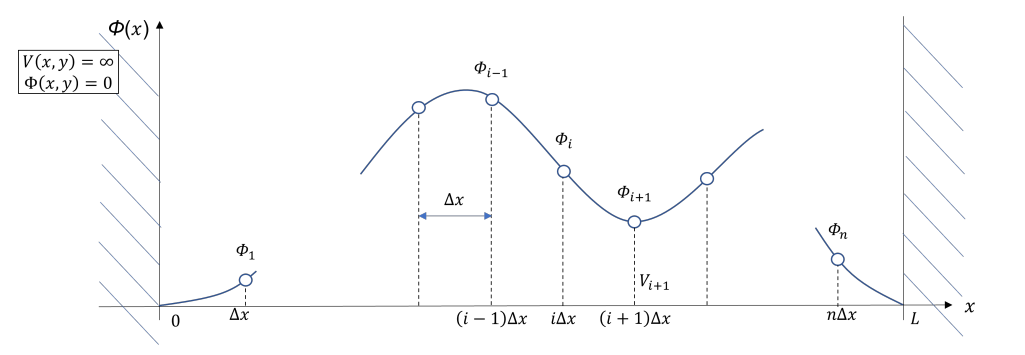
\includegraphics[width=1.1\linewidth]{images/一次元.png} \\
      図4.1:実空間差分法
    \end{center}
    
    すると,1階微分は前進・後退差分により以下のように近似される.
  \[
  \begin{array}{l@{\hspace{1cm}}l}
  \displaystyle
  \left.\frac{d\phi}{dx}\right|_{x = (i+\frac{1}{2})\Delta x}
  \approx \frac{\phi_{i+1} - \phi_{i}}{\Delta x}
  &
  \displaystyle
  \left.\frac{d\phi}{dx}\right|_{x = (i-\frac{1}{2})\Delta x}
  \approx \frac{\phi_{i} - \phi_{i-1}}{\Delta x}
  \end{array}\]
    \end{frame}
    
    \begin{frame}{演習①\quad 2階微分の導出}
    先ほどの1階微分の近似式を用いて,$x = i\Delta x$における2階微分ではどのような近似式になるかを導出せよ.
    
    \bigskip
    $$
    \left. \frac{d^2 \phi}{dx^2} \right|_{x = i\Delta x}
    \approx \quad ?
    $$

    \end{frame}

    \begin{frame}{演習①\quad 2階微分の導出 解答}

      
      \bigskip
      
      \textbf{解答}:
      1階微分の近似式同士で差分を取ることで以下のように求められる:
      % \begin{equation}
      % \left. \frac{d^2 \phi}{dx^2} \right|_{x = i\Delta x}
      % =\frac{d}{dx}\left(\left. \frac{d \phi}{dx} \right)\right|_{x = i\Delta x}\\
      % \approx \frac{\left.\frac{d\phi}{dx}\right|_{x = (i+\frac{1}{2})\Delta x} - \left.\frac{d\phi}{dx}\right|_{x = (i+\frac{1}{2})\Delta x}}{\Delta x}
      % \end{equation}

      $$
      \left. \frac{d^2 \phi}{dx^2} \right|_{x = i\Delta x}
      \approx \frac{\phi_{i+1} - 2\phi_i + \phi_{i-1}}{(\Delta x)^2}
      $$
      \end{frame}

  \begin{frame}{2次元シュレディンガー方程式への応用}

    シュレディンガー方程式は見ての通り,
    $$
    \left[ -\frac{1}{2} \nabla^2 + V( \mathbf{r} ) \right] \phi = E \phi
    $$
    偏微分方程式であるが,実空間差分法を使うと行列の固有値問題に落とし込める.
    
    まず,二次元空間を格子状メッシュで分割し,各点で波動関数 $\phi(x,y)$ を定義する.差分法を使うと,ラプラシアンは以下のように近似される:
    
    $$
    \nabla^2 \phi(x,y)\big|_{(x=i\Delta,y=j \Delta)} 
    \approx \frac{\phi_{i+1,j} + \phi_{i-1,j} + \phi_{i,j+1} + \phi_{i,j-1} - 4\phi_{i,j}}{(\Delta )^2}
    $$
    
    差分化した2次元シュレディンガー方程式:
    $$
    -\frac{1}{2\Delta^2} (\phi_{i+1,j} + \phi_{i-1,j} + \phi_{i,j+1} + \phi_{i,j-1} - 4\phi_{i,j} ) + V_{i,j} \phi_{i,j} = E \phi_{i,j}
    $$
    \end{frame}
    
\begin{frame}{演習②\quad ハミルトニアン行列の構築}
      \setlength{\leftskip}{-1.5em}   % 左余白を詰める
    \setlength{\rightskip}{-1.5em}
    差分化された2次元シュレディンガー方程式は,連立斉次方程式であるため行列へと落とし込むことが出来る.以下の行列のハミルトニアン行列部分の空欄を埋めよ.
    \vspace{0.5em}
    
    \begin{minipage}{0.5\textwidth}
    \scriptsize
    $$
    \underbrace{
    \begin{pmatrix}
    \_ & \_ & \_ & \_ & \_ & \_ & \_ & \_ & \_ \\
    \_ & \_ & \_ & \_ & \_ & \_ & \_ & \_ & \_ \\
    \_ & \_ & \_ & \_ & \_ & \_ & \_ & \_ & \_ \\
    \hline
    \_ & \_ & \_ & \_ & \_ & \_ & \_ & \_ & \_ \\
    \_ & \_ & \_ & \_ & \_ & \_ & \_ & \_ & \_ \\
    \_ & \_ & \_ & \_ & \_ & \_ & \_ & \_ & \_ \\
    \hline
    \_ & \_ & \_ & \_ & \_ & \_ & \_ & \_ & \_ \\
    \_ & \_ & \_ & \_ & \_ & \_ & \_ & \_ & \_ \\
    \_ & \_ & \_ & \_ & \_ & \_ & \_ & \_ & \_ 
    \end{pmatrix}
    }_{\text{ハミルトニアン行列}}
    \begin{pmatrix}
    \phi_{1,1} \\ \phi_{1,2} \\ \phi_{1,3} \\
    \hline
    \phi_{2,1} \\ \phi_{2,2} \\ \phi_{2,3} \\
    \hline
    \phi_{3,1} \\ \phi_{3,2} \\ \phi_{3,3}
    \end{pmatrix}
    =
    E
    \begin{pmatrix}
    \phi_{1,1} \\ \phi_{1,2} \\ \phi_{1,3} \\
    \hline
    \phi_{2,1} \\ \phi_{2,2} \\ \phi_{2,3} \\
    \hline
    \phi_{3,1} \\ \phi_{3,2} \\ \phi_{3,3}
    \end{pmatrix}
        $$
  \end{minipage}
  \hfill
  \begin{minipage}{0.36\textwidth}
  \centering
  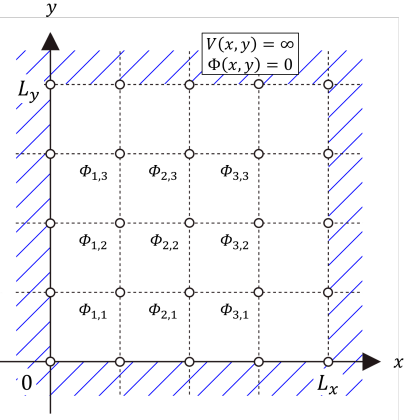
\includegraphics[width=1\linewidth]{images/二次元.png} \\
  \hspace{0.3em}
  {\scriptsize 図4.2:3×3格子における2次元差分のイメージ}
  \end{minipage}
  \end{frame}
       
\begin{frame}{演習②\quad 解答}
    連立斉次方程式に落とし込むことで以下のようになる.
\begin{flushleft}    
    {\tiny
    \[
    \left[
    \begin{array}{@{\hskip 1pt}c@{\hskip 1pt}c@{\hskip 1pt}c@{\hskip 3pt}
                  @{\hskip 1pt}c@{\hskip 1pt}c@{\hskip 1pt}c@{\hskip 3pt}
                  @{\hskip 1pt}c@{\hskip 1pt}c@{\hskip 1pt}c}
    \frac{-4}{2\Delta^2}+V_{1,1} &  \frac{1}{2\Delta^2} & 0 &  \frac{1}{2\Delta^2} & 0 & 0 & 0 & 0 & 0 \\
    \frac{1}{2\Delta^2} & \frac{-4}{2\Delta^2}+V_{1,2} &  \frac{1}{2\Delta^2} & 0 &  \frac{1}{2\Delta^2} & 0 & 0 & 0 & 0 \\
    0 &  \frac{1}{2\Delta^2} & \frac{-4}{2\Delta^2}+V_{1,3} & 0 & 0 &  \frac{1}{2\Delta^2} & 0 & 0 & 0 \\
    \rule{0pt}{1.2em} \\  % ← 空行で区切る
    \frac{1}{2\Delta^2} & 0 & 0 & \frac{-4}{2\Delta^2}+V_{2,1} &  \frac{1}{2\Delta^2} & 0 &  \frac{1}{2\Delta^2} & 0 & 0 \\
    0 &  \frac{1}{2\Delta^2} & 0 &  \frac{1}{2\Delta^2} & \frac{-4}{2\Delta^2}+V_{2,2} &  \frac{1}{2\Delta^2} & 0 &  \frac{1}{2\Delta^2} & 0 \\
    0 & 0 &  \frac{1}{2\Delta^2} & 0 &  \frac{1}{2\Delta^2} & \frac{-4}{2\Delta^2}+V_{2,3} & 0 & 0 &  \frac{1}{2\Delta^2} \\
    \rule{0pt}{1.2em} \\
    0 & 0 & 0 &  \frac{1}{2\Delta^2} & 0 & 0 & \frac{-4}{2\Delta^2}+V_{3,1} &  \frac{1}{2\Delta^2} & 0 \\
    0 & 0 & 0 & 0 &  \frac{1}{2\Delta^2} & 0 &  \frac{1}{2\Delta^2} & \frac{-4}{2\Delta^2}+V_{3,2} &  \frac{1}{2\Delta^2}1 \\
    0 & 0 & 0 & 0 & 0 &  \frac{1}{2\Delta^2} & 0 &  \frac{1}{2\Delta^2} & \frac{-4}{2\Delta^2}+V_{3,3}
    \end{array}
    \right]
    \]
    \normalsize}
\end{flushleft}
    この行列を対角化することで,固有エネルギー(固有値)と波動関数(固有ベクトル)を求めることが出来る.
    

\end{frame}
    
\begin{frame}{5. 計算結果の解析}
ハイブリッドポテンシャルの数値解を計算するファイルを実行して,
調和ポテンシャル,円筒ポテンシャルの解析解と比較する.
  \begin{itemize}
    \item \textbf{数値解}:  \\
    \rightarrow ハイブリッドポテンシャル
    \item \textbf{解析解}:  \\
    \rightarrow 調和ポテンシャル \\
    \rightarrow 円筒ポテンシャル 
    \item \textbf{準位図比較}:  \\
    \rightarrow 調和ポテンシャル,円筒ポテンシャルの解析解とハイブリッドポテンシャルの数値解
    の準位図を比較する.
    \item \textbf{閉じ込め強度依存性}:  \\
    \rightarrow 閉じ込め強度$\omega$を変化させて,調和ポテンシャル解析解と
    ハイブリッドポテンシャル数値解を比較する
  \end{itemize}
\end{frame}

\begin{frame}{5.1 数値解}
  ノートブックを実行して下さい
\end{frame} 

  \begin{frame}{}
  \textbf{解析解①\quad 調和ポテンシャル}

          調和ポテンシャル下における波動関数解析解は次のようになる\ $(n = 0,1,2,\dots)$,$(l = 0,\pm1,\pm2,\dots)$:
              \vspace{-0.0em}       
        \begin{equation*}
        \phi_{n}^{\,l}(z,\theta)
        = \frac{1}{\sqrt{\pi}}
        \sqrt{\frac{n!}{(n + |l|)!}}\,
        z^{\,|l|}\,e^{-z^2/2}\,
        L_{n}^{(|l|)}\bigl(z^2\bigr)\,
        \exp\bigl(i\,l\,\theta\bigr),
        z = \sqrt{\frac{m\,\omega}{\hbar}}\,r.
        \end{equation*}
        
            \vspace{-2.5em}        

        \begin{columns}
          \column{0.4\textwidth}
          ここで $L_{n}^{(|l|)}$ はラゲールの陪多項式を表す.\\

          また,そのエネルギー固有値は
          \begin{equation*}
          E_{n}^{\,l} = \hbar\,\omega\,\bigl(2\,n + |l| + 1\bigr).
          \end{equation*}

          \column{0.6\textwidth}
          \begin{center}
            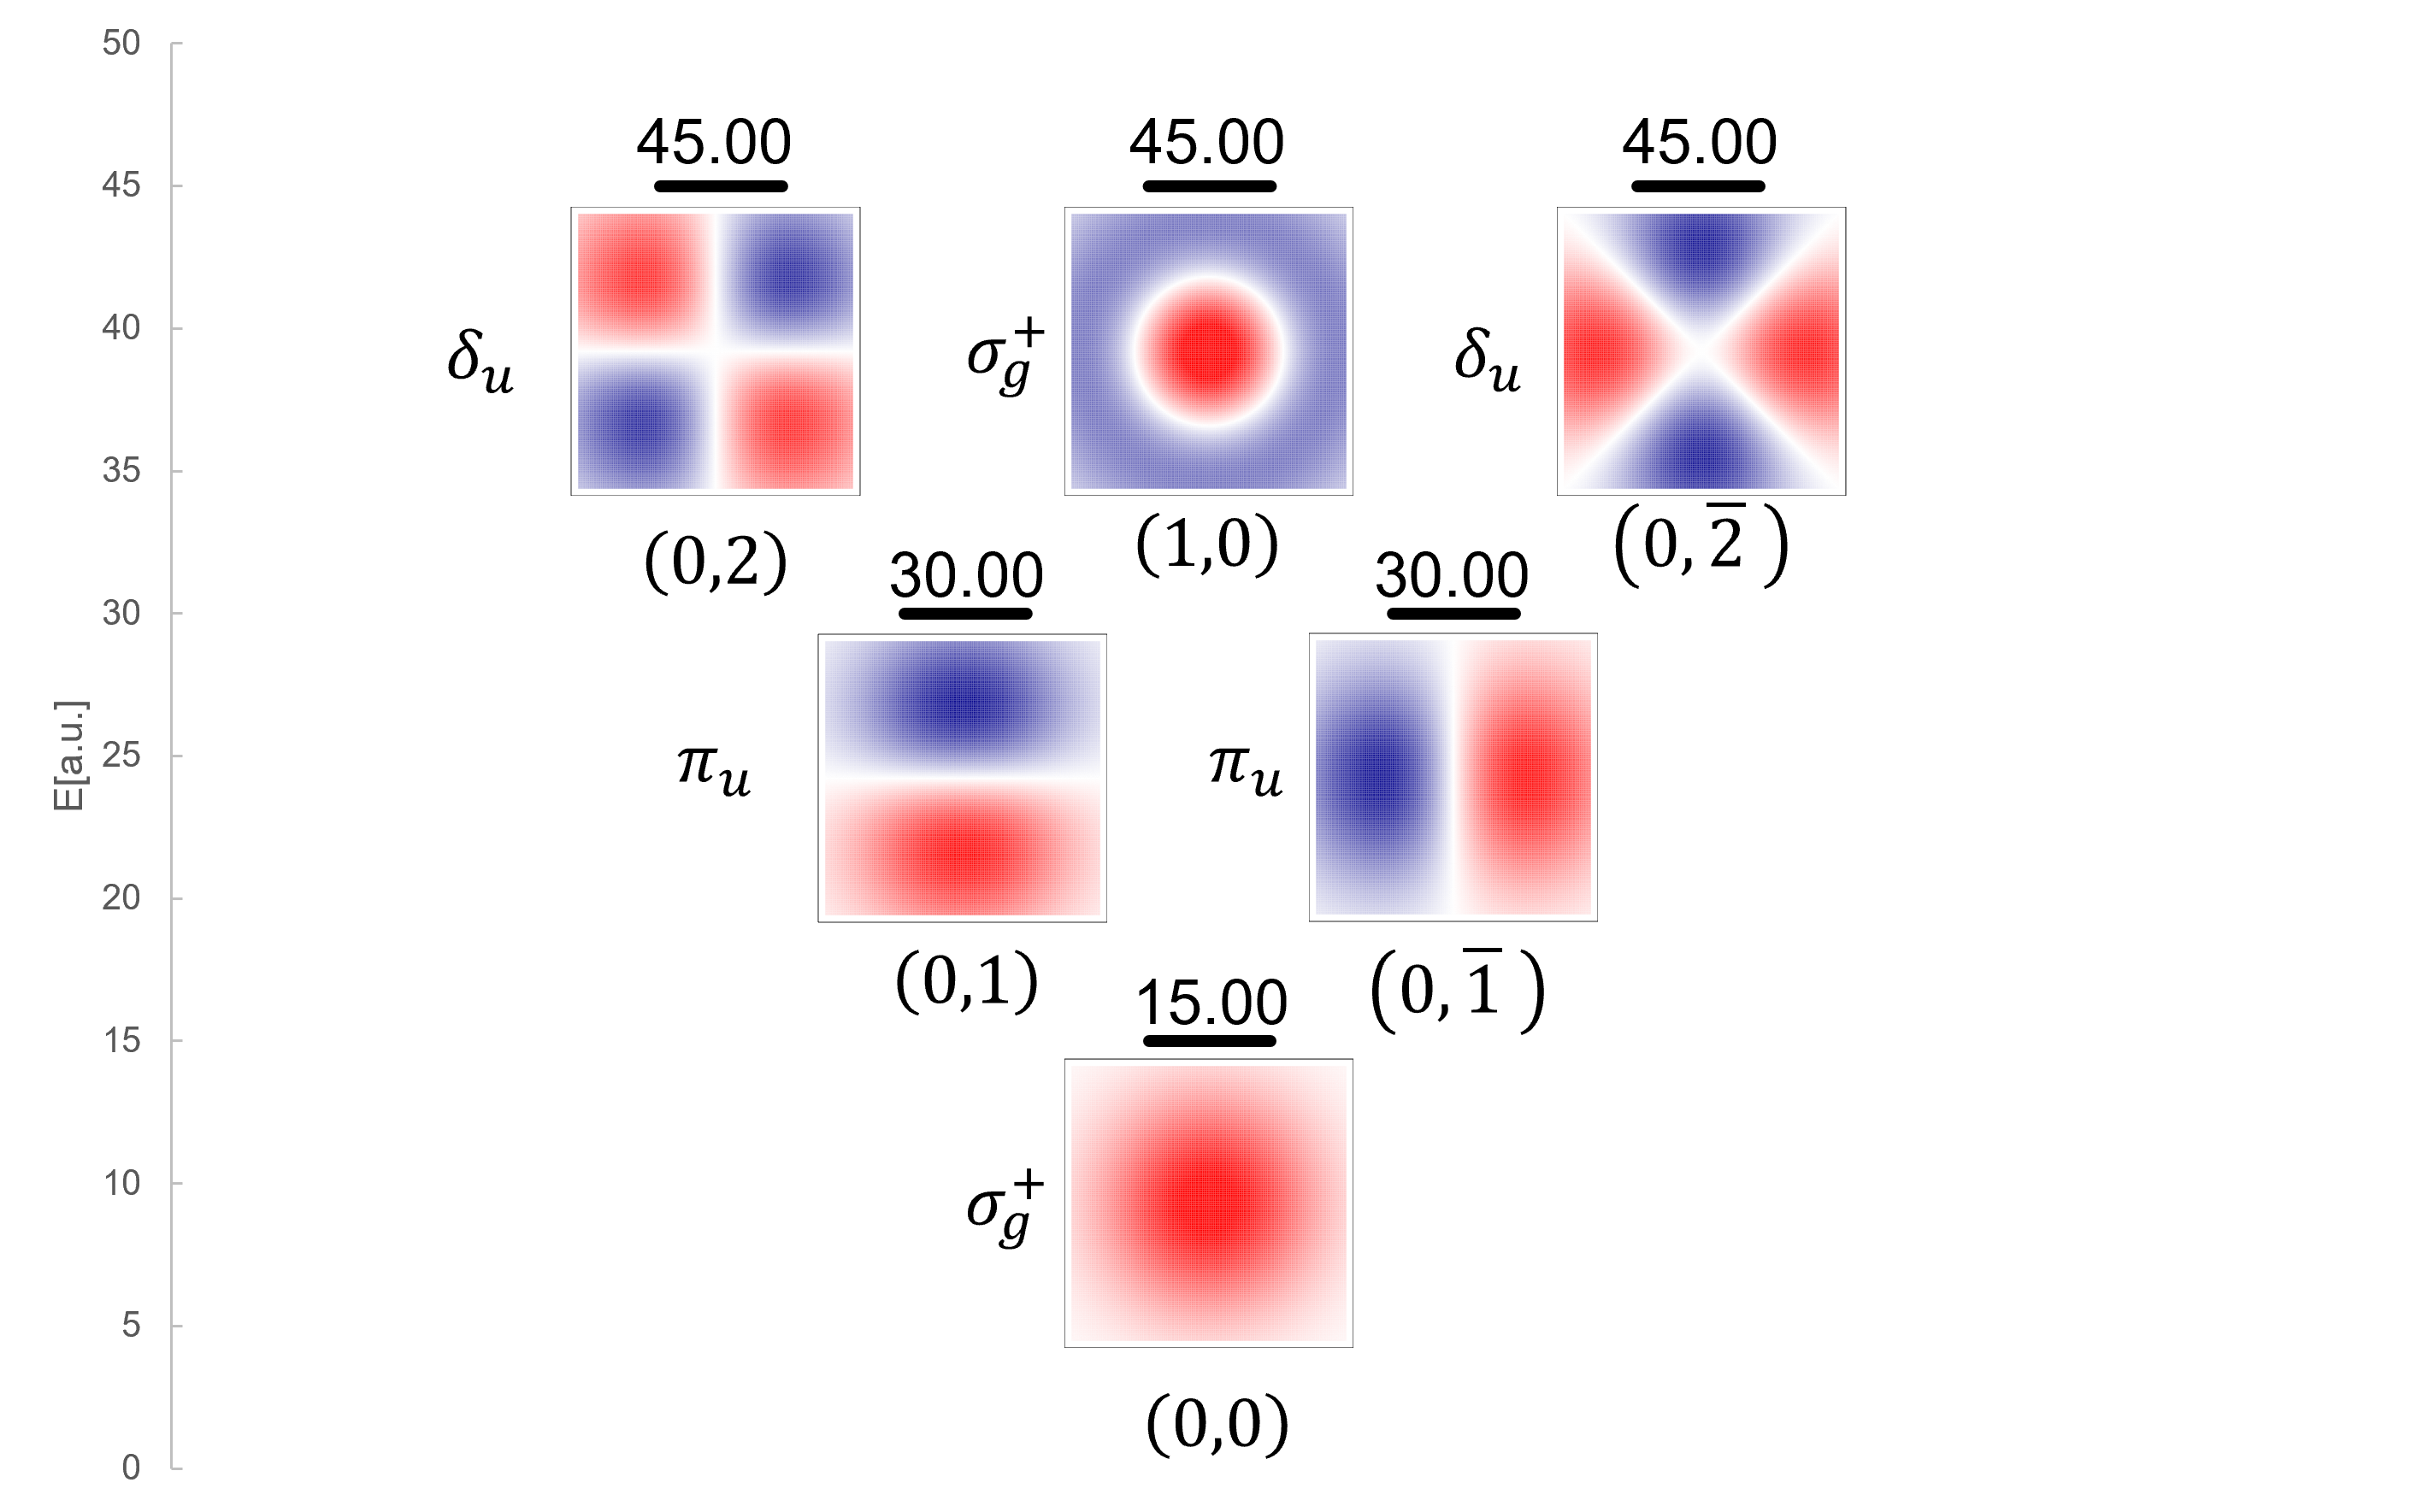
\includegraphics[width=1.4\linewidth]{images/調和準位図.png} \\
            \vspace{0.5em}
            {\small 図5.1:調和解析解準位図}
          \end{center}
        \end{columns}

        
        % \column{0.6\textwidth}
        % \begin{center}
        %   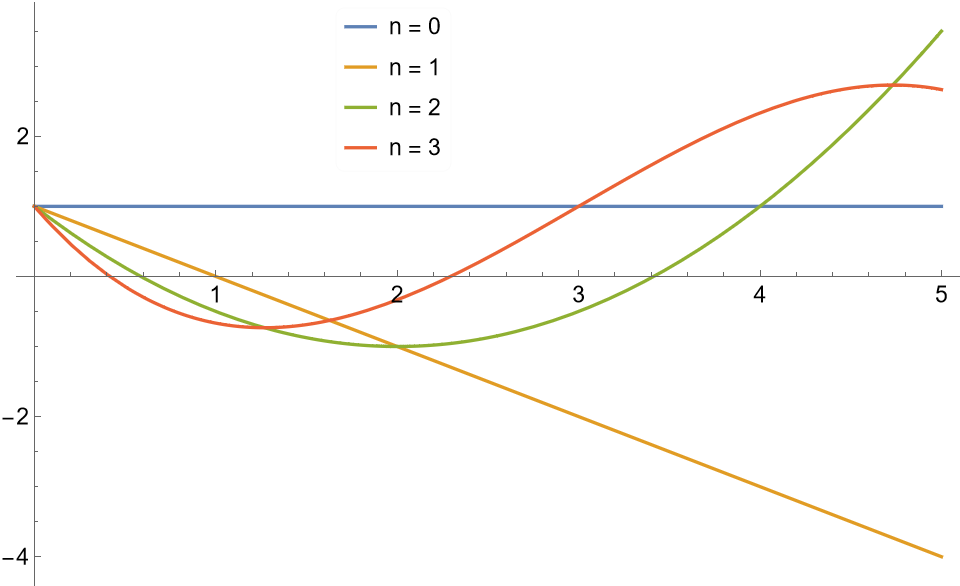
\includegraphics[width=0.65\linewidth]{images/ラゲール.png} \\
        %   図5.4:ラゲール陪多項式の振る舞い
        % \end{center}
        % \end{columns}
  
  \end{frame}
  
  \begin{frame}{}
    \textbf{解析解②\quad 円筒ポテンシャル}    

  円筒ポテンシャル下における波動関数解析解は次のようになる\ $(n = 0,1,2,\dots)$,$(l = 0,\pm1,\pm2,\dots)$:
     \vspace{-0.0em}  
  \begin{equation*}
  \phi_{n}^{\,l}(r,\theta)
  = \frac{1}{\sqrt{\pi}\,r_0\,\lvert J_{|l|+1}(Z_{|l|,n+1})\rvert}\,
  J_{|l|}\!\Bigl(Z_{|l|,n+1}\,\frac{r}{r_0}\Bigr)
  \,\exp\bigl(i\,l\,\theta\bigr).
  \end{equation*}
   \vspace{-2.5em}  
          \begin{columns}
          \column{0.4\textwidth}

          ここで $J_{|l|}$ は第一種ベッセル関数をあらわし,$Z_{|l|,n+1}$ はそのn+1番目の零点である.\\
          また,そのエネルギー固有値は
          \begin{equation*}
          E_{n}^{\,l} 
          = \frac{\hbar^2}{2\,m}\,\Bigl(\frac{Z_{|l|,n+1}}{r_0}\Bigr)^2\,.
          \end{equation*}


          \column{0.6\textwidth}
          \begin{center}
            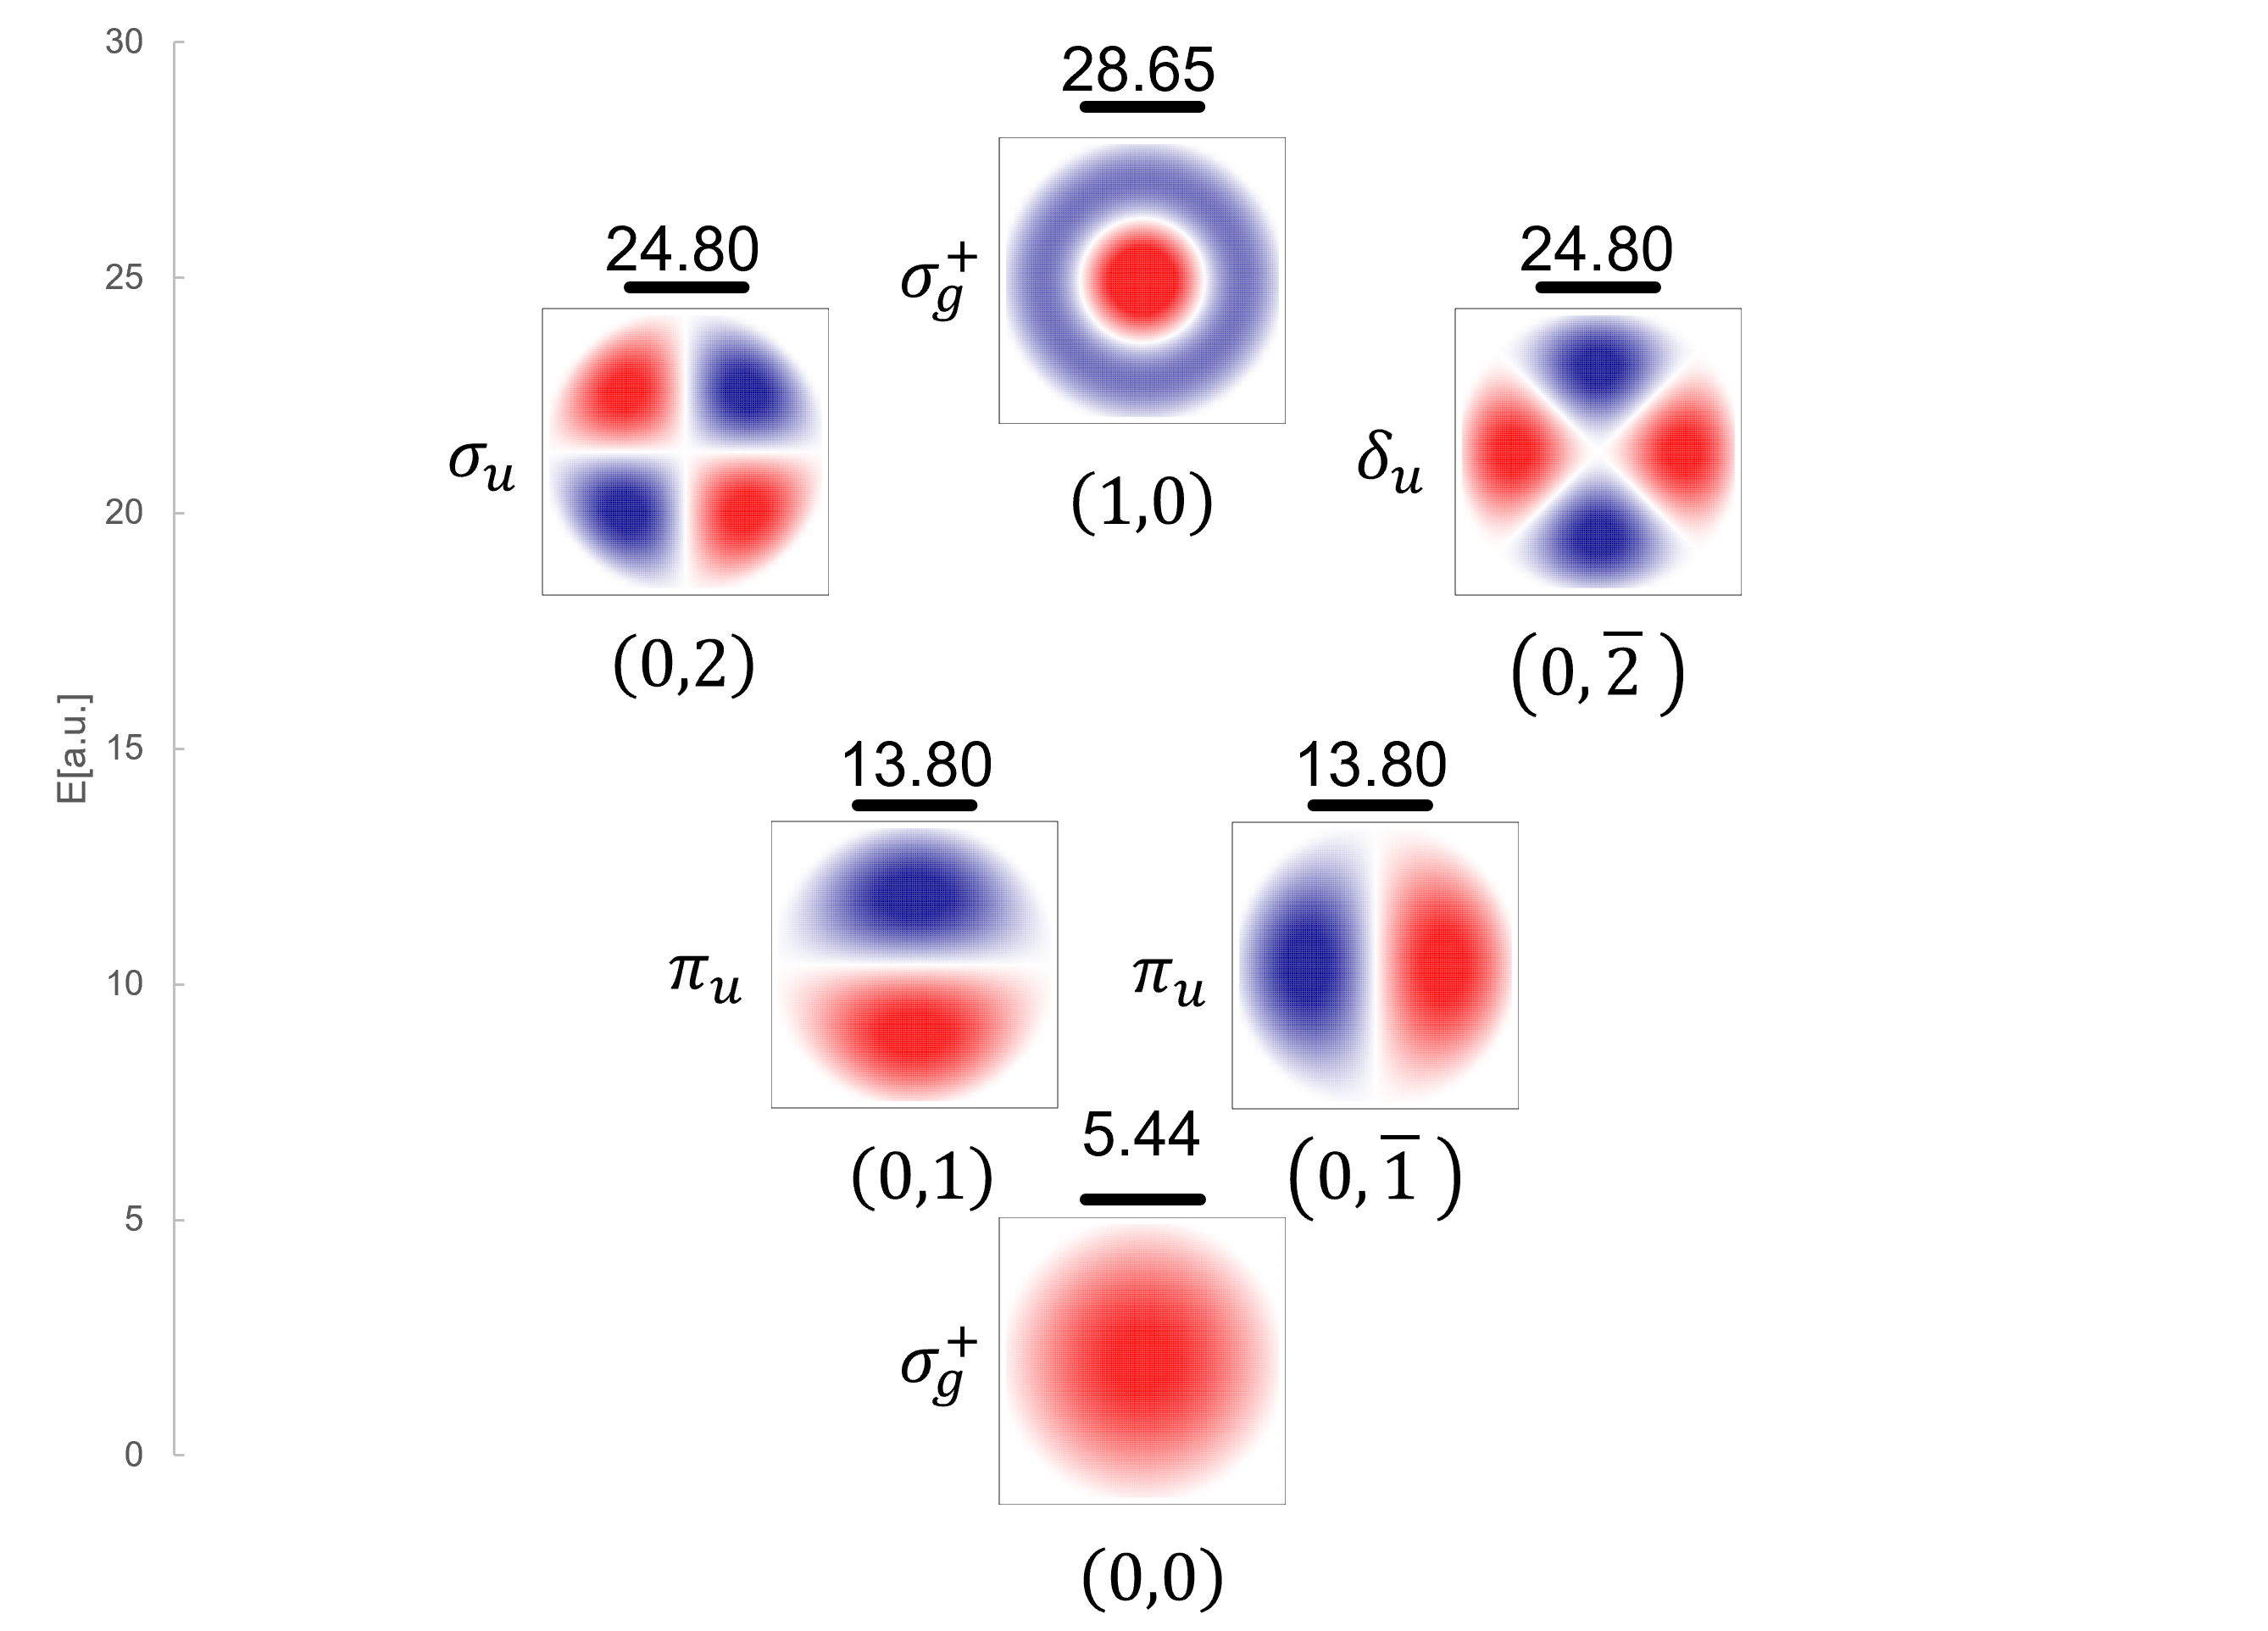
\includegraphics[width=1.28\linewidth]{images/円筒準位図.png} \\
            \vspace{0.5em}
            {\small 図5.2:円筒解析解準位図}
          \end{center}
        \end{columns}


  % また,そのエネルギー固有値は

  % \begin{equation*}
  % E_{n}^{\,l} 
  % = \frac{\hbar^2}{2\,m}\,\Bigl(\frac{Z_{|l|,n+1}}{r_0}\Bigr)^2\,.
  % \end{equation*}
  
  % ここで $J_{|l|}$ は第一種ベッセル関数,$Z_{|l|,n+1}$ はそのゼロ点(n+1 番目)を表す.
  
  % \begin{columns}
  % \column{0.48\textwidth}
  % \begin{center}
  %   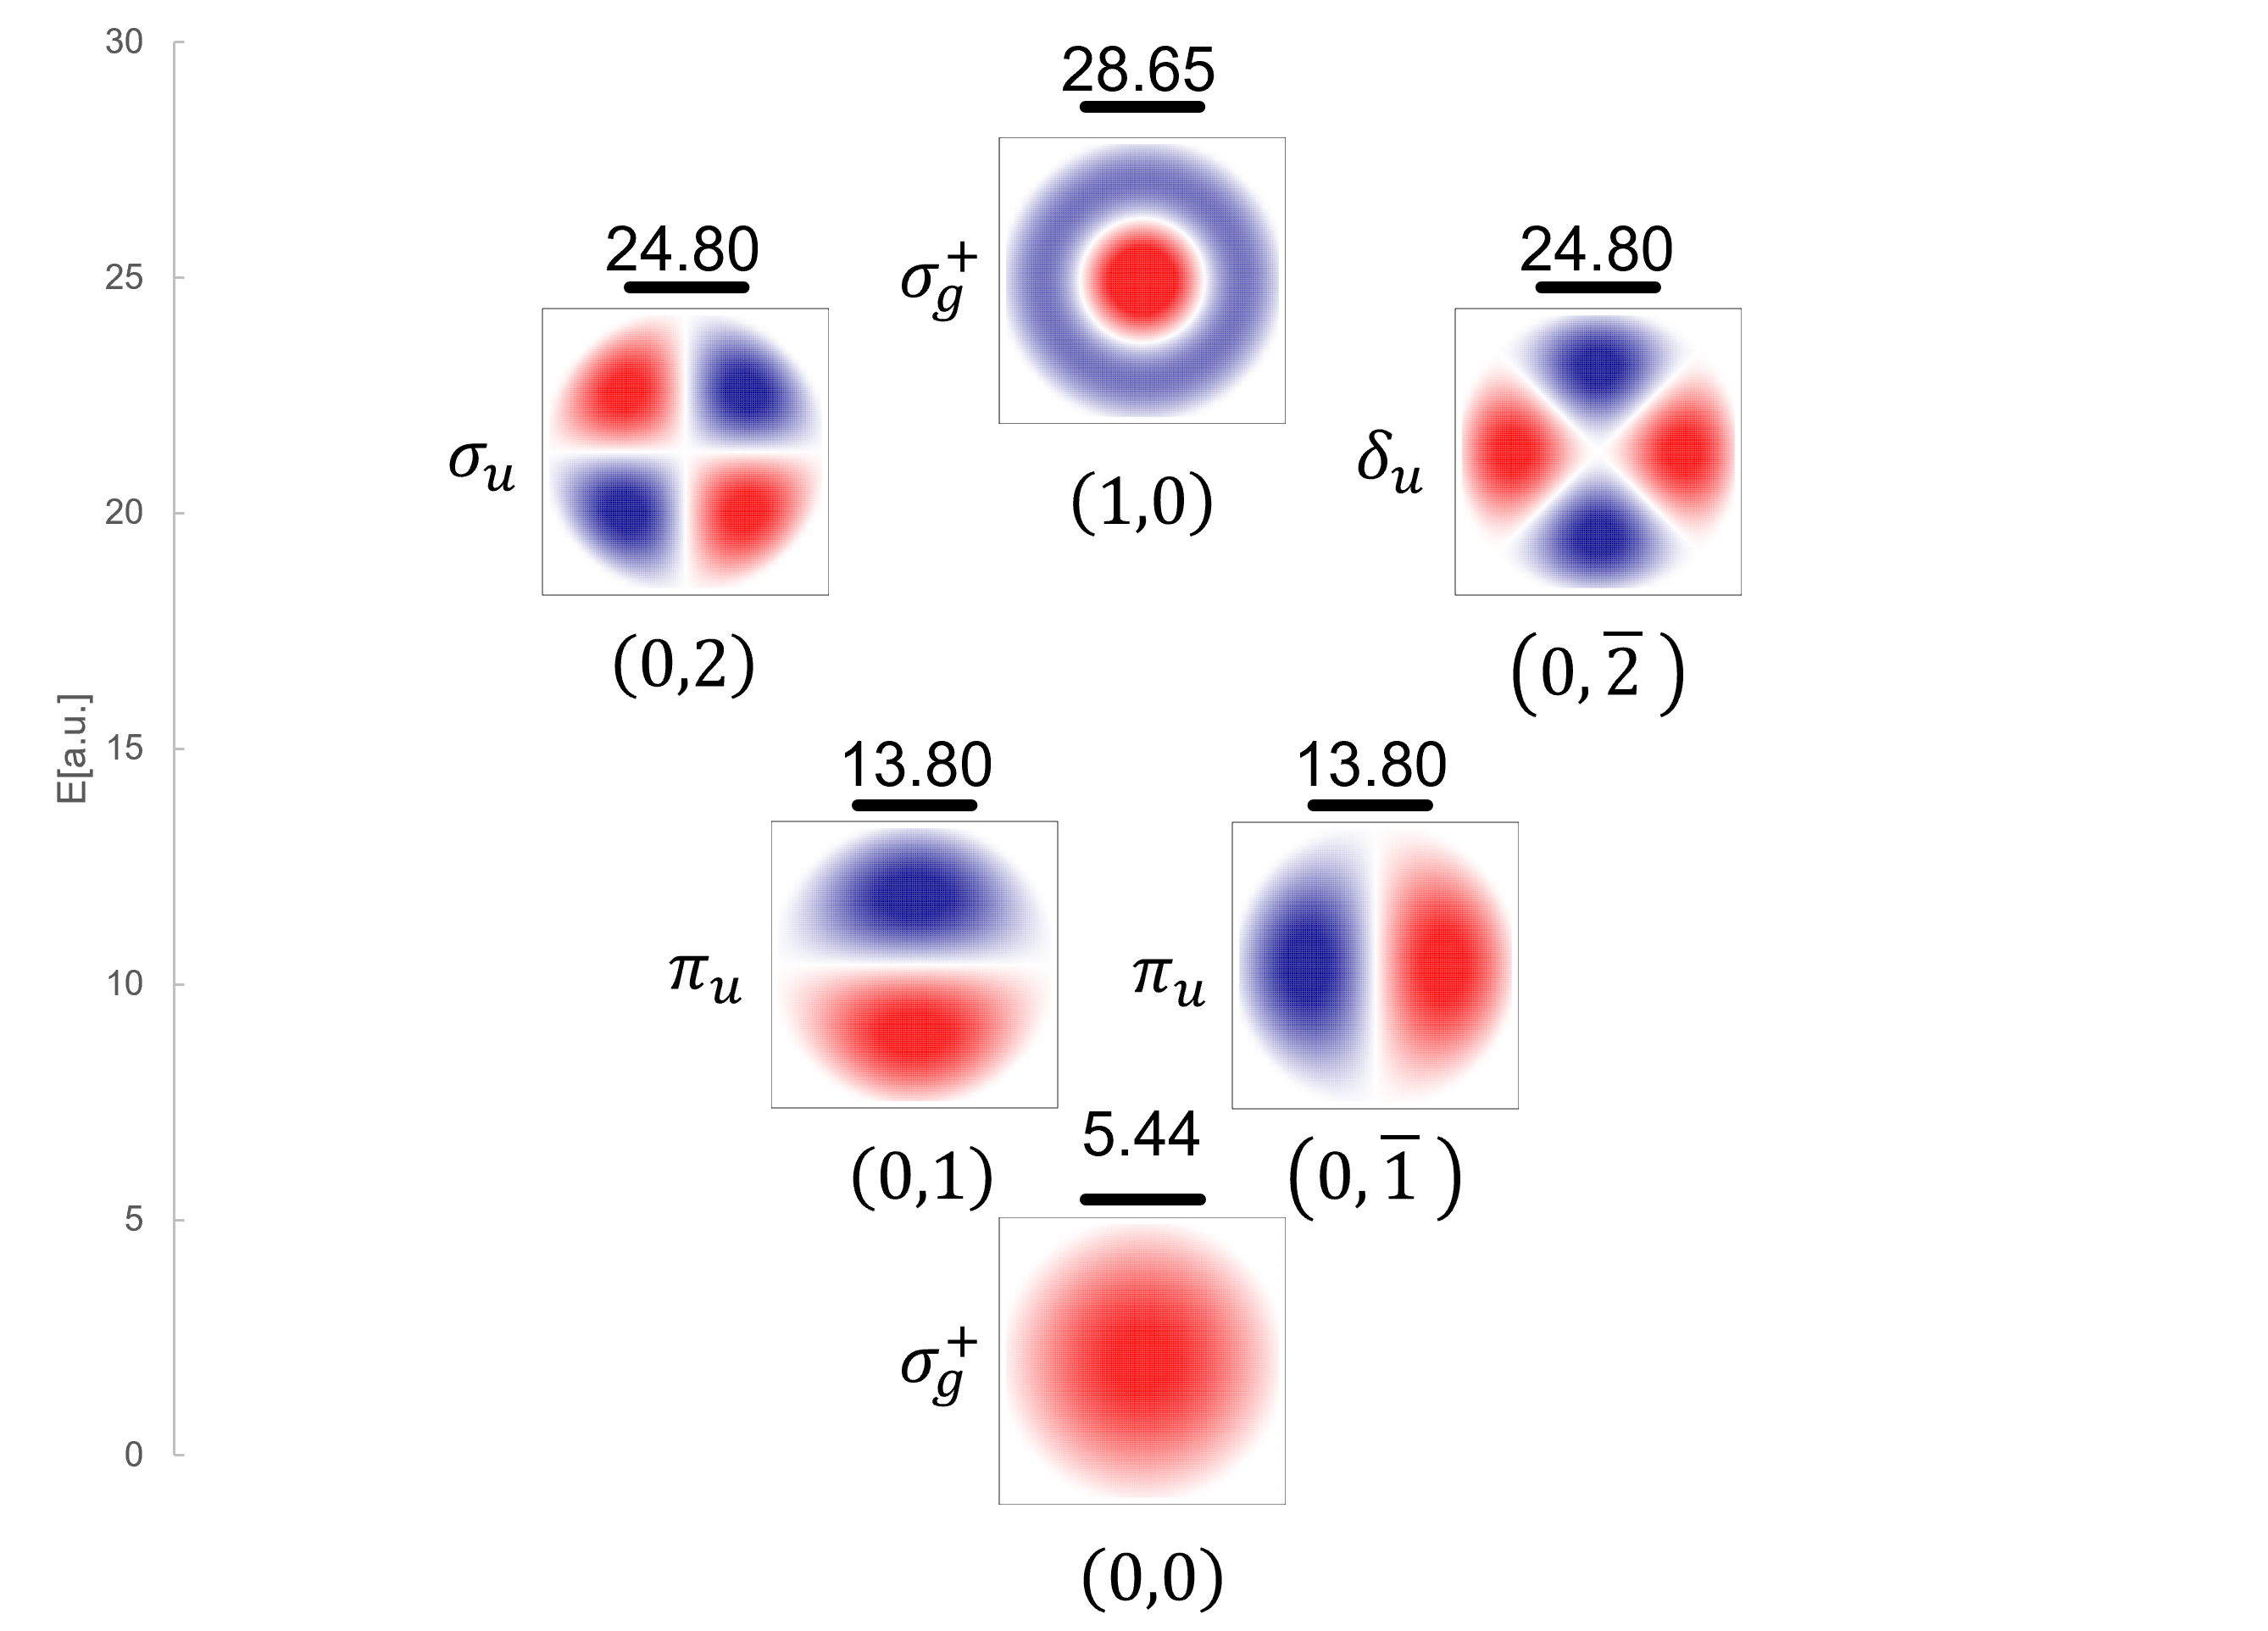
\includegraphics[width=0.45\linewidth]{images/円筒準位図.png} \\
  %   図5.1:円筒解析解準位図
  % \end{center}
  
  % \column{0.48\textwidth}
  % \begin{center}
  %   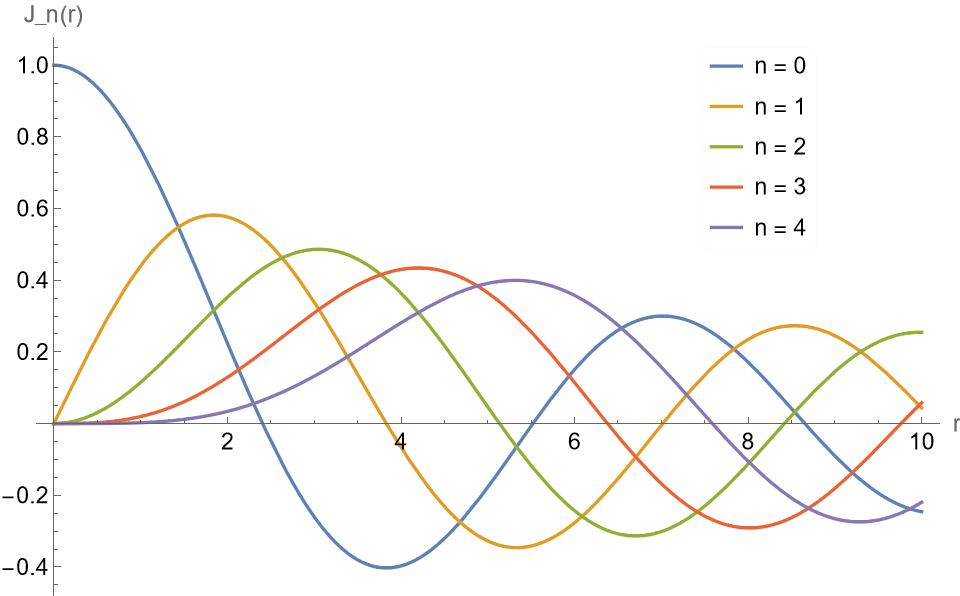
\includegraphics[width=0.50\linewidth]{images/ベッセル.png} \\
  %   図5.2:ベッセル関数の振る舞い
  % \end{center}
  % \end{columns}
  

  \end{frame}
 \begin{frame}{5.2 解析解と数値解の準位図
    比較}
  \textbf{演習③\quad 計算結果の解析}
        \begin{itemize}
          \item 円筒ポテンシャルの準位図(解析解)と調和ポテンシャルの準位図(解析解)とを比較し考察せよ.また,量子数と波動関数の関係性についても述べよ。
          \item ハイブリッドポテンシャルの準位図(数値解)と,円筒ポテンシャル,及び,調和ポテンシャルの準位図(解析解)との類似性について考察せよ.
        \end{itemize}
        

        
        \begin{columns}[t]

          \column{0.32\textwidth}
          \begin{center}
            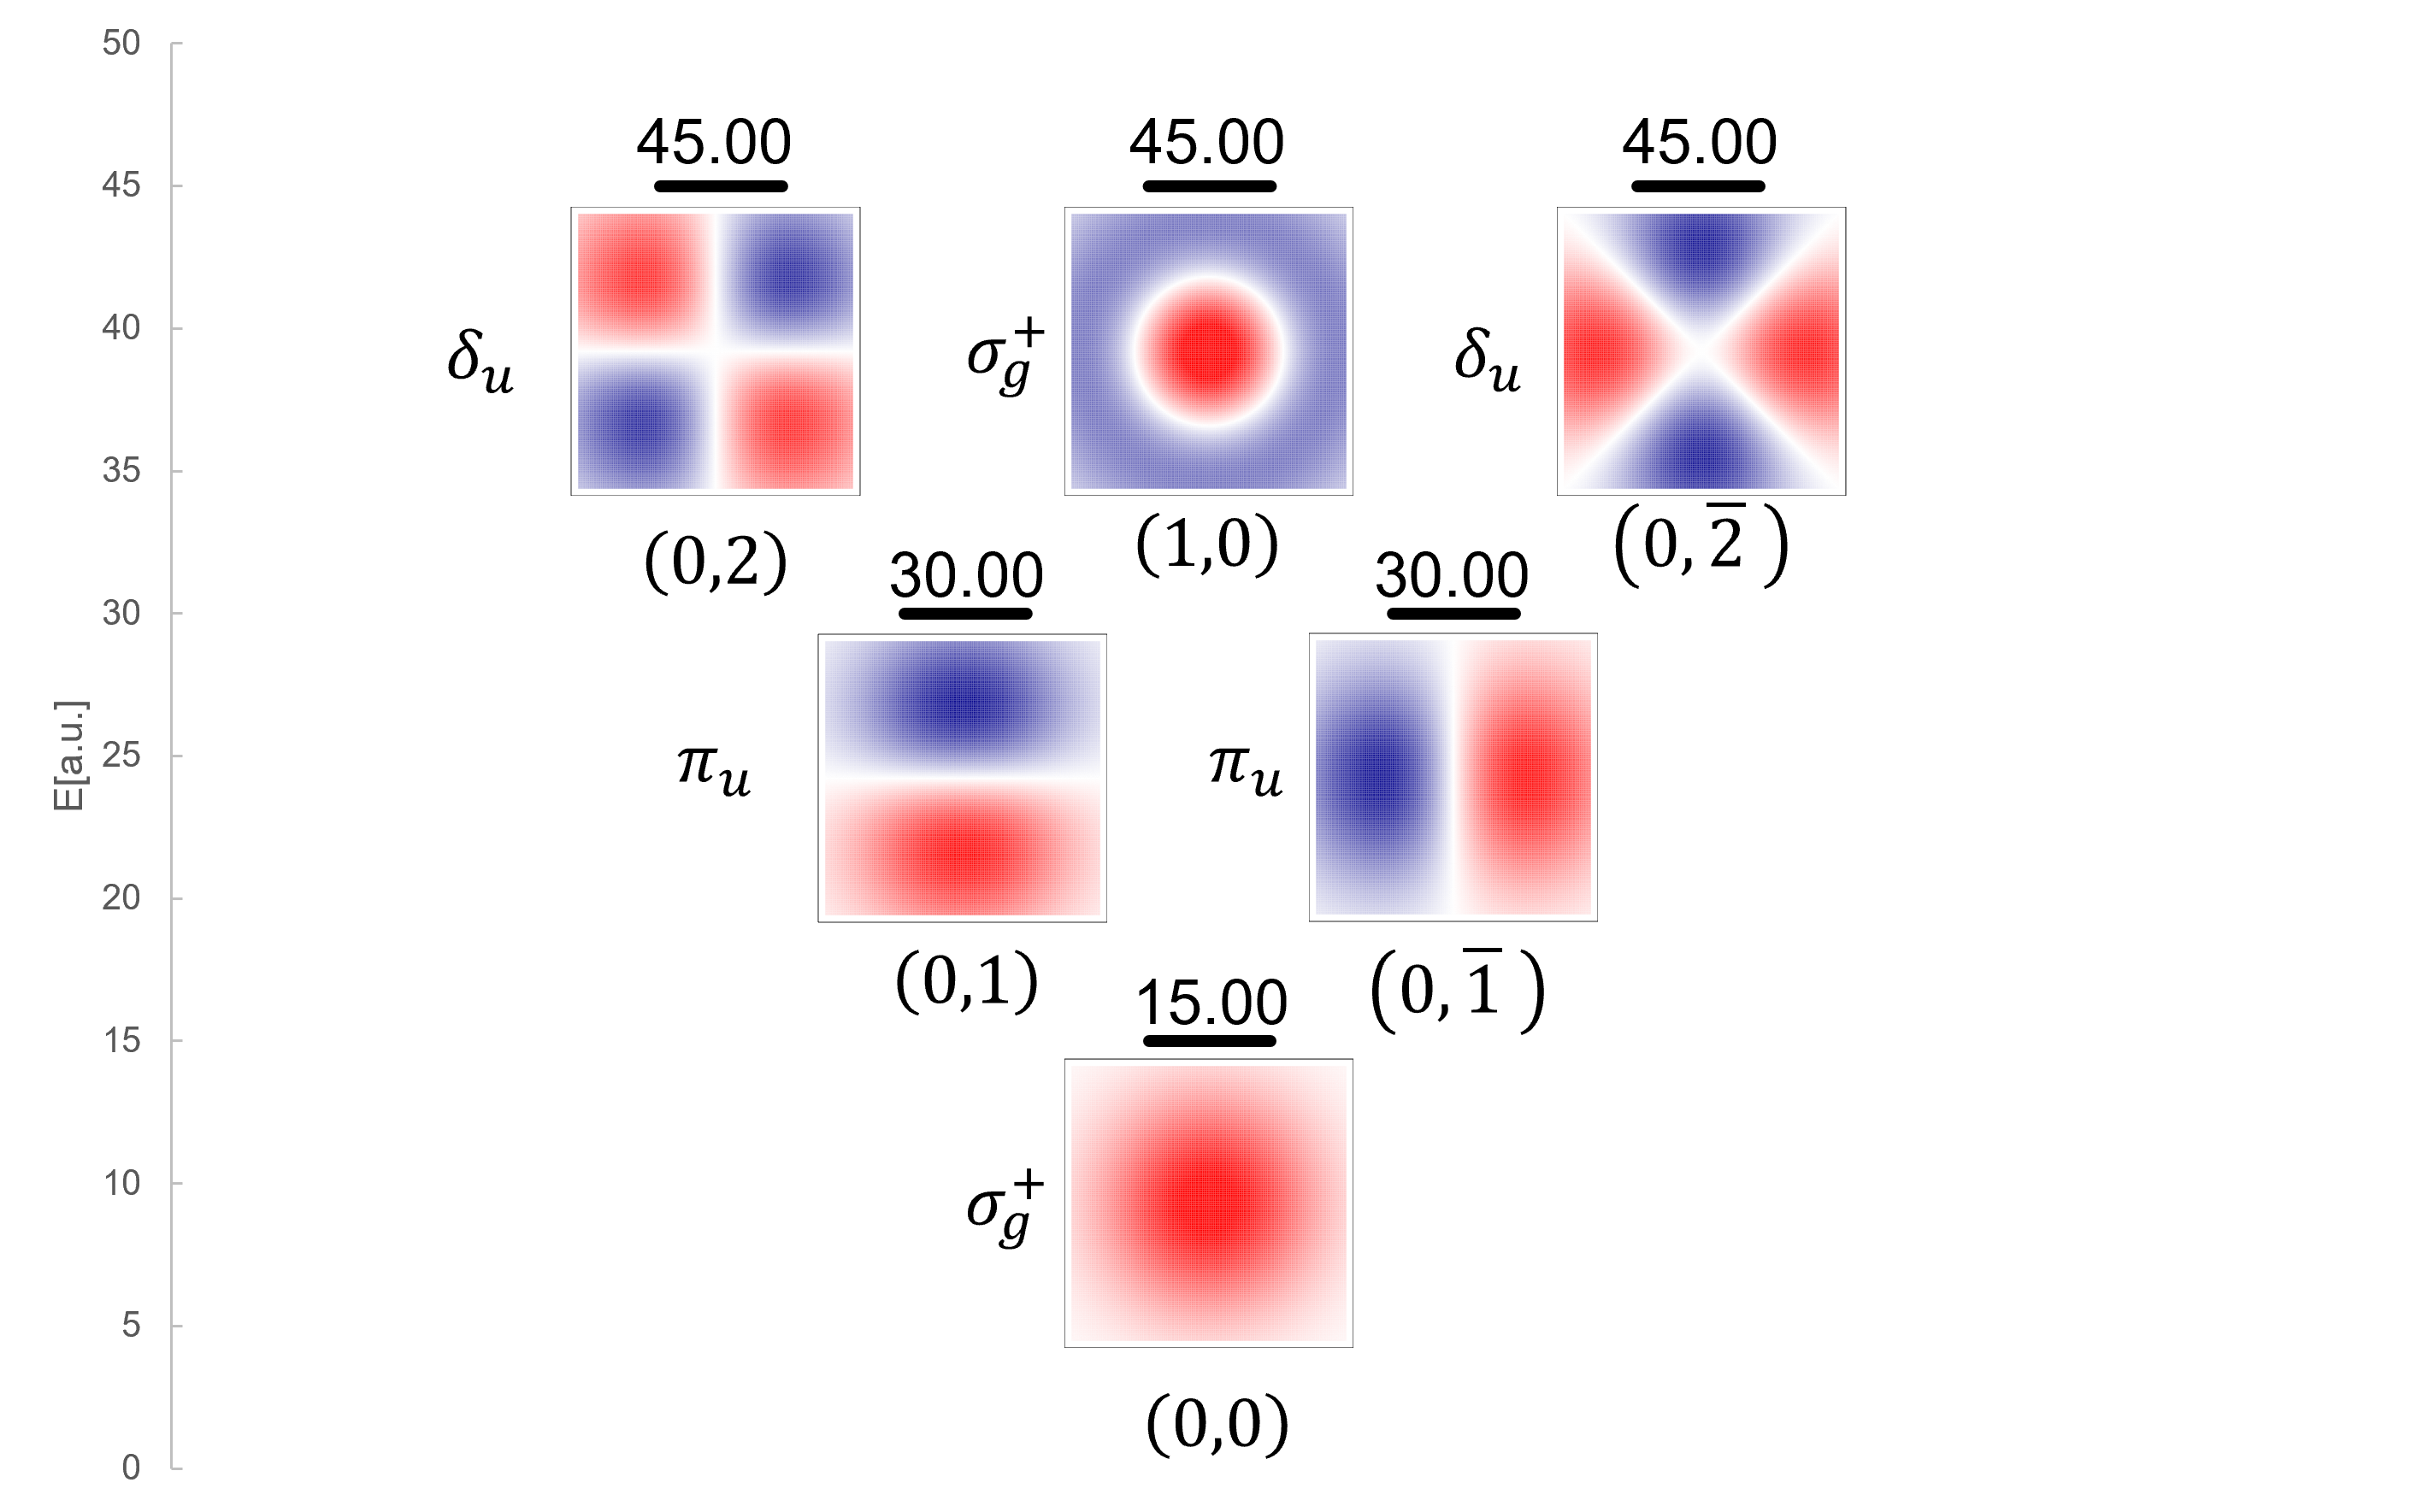
\includegraphics[width=1.30\linewidth]{images/調和準位図.png} \\
            \scriptsize 図5.3:調和解析解準位図
          \end{center}


          \column{0.32\textwidth}
          \begin{center}
            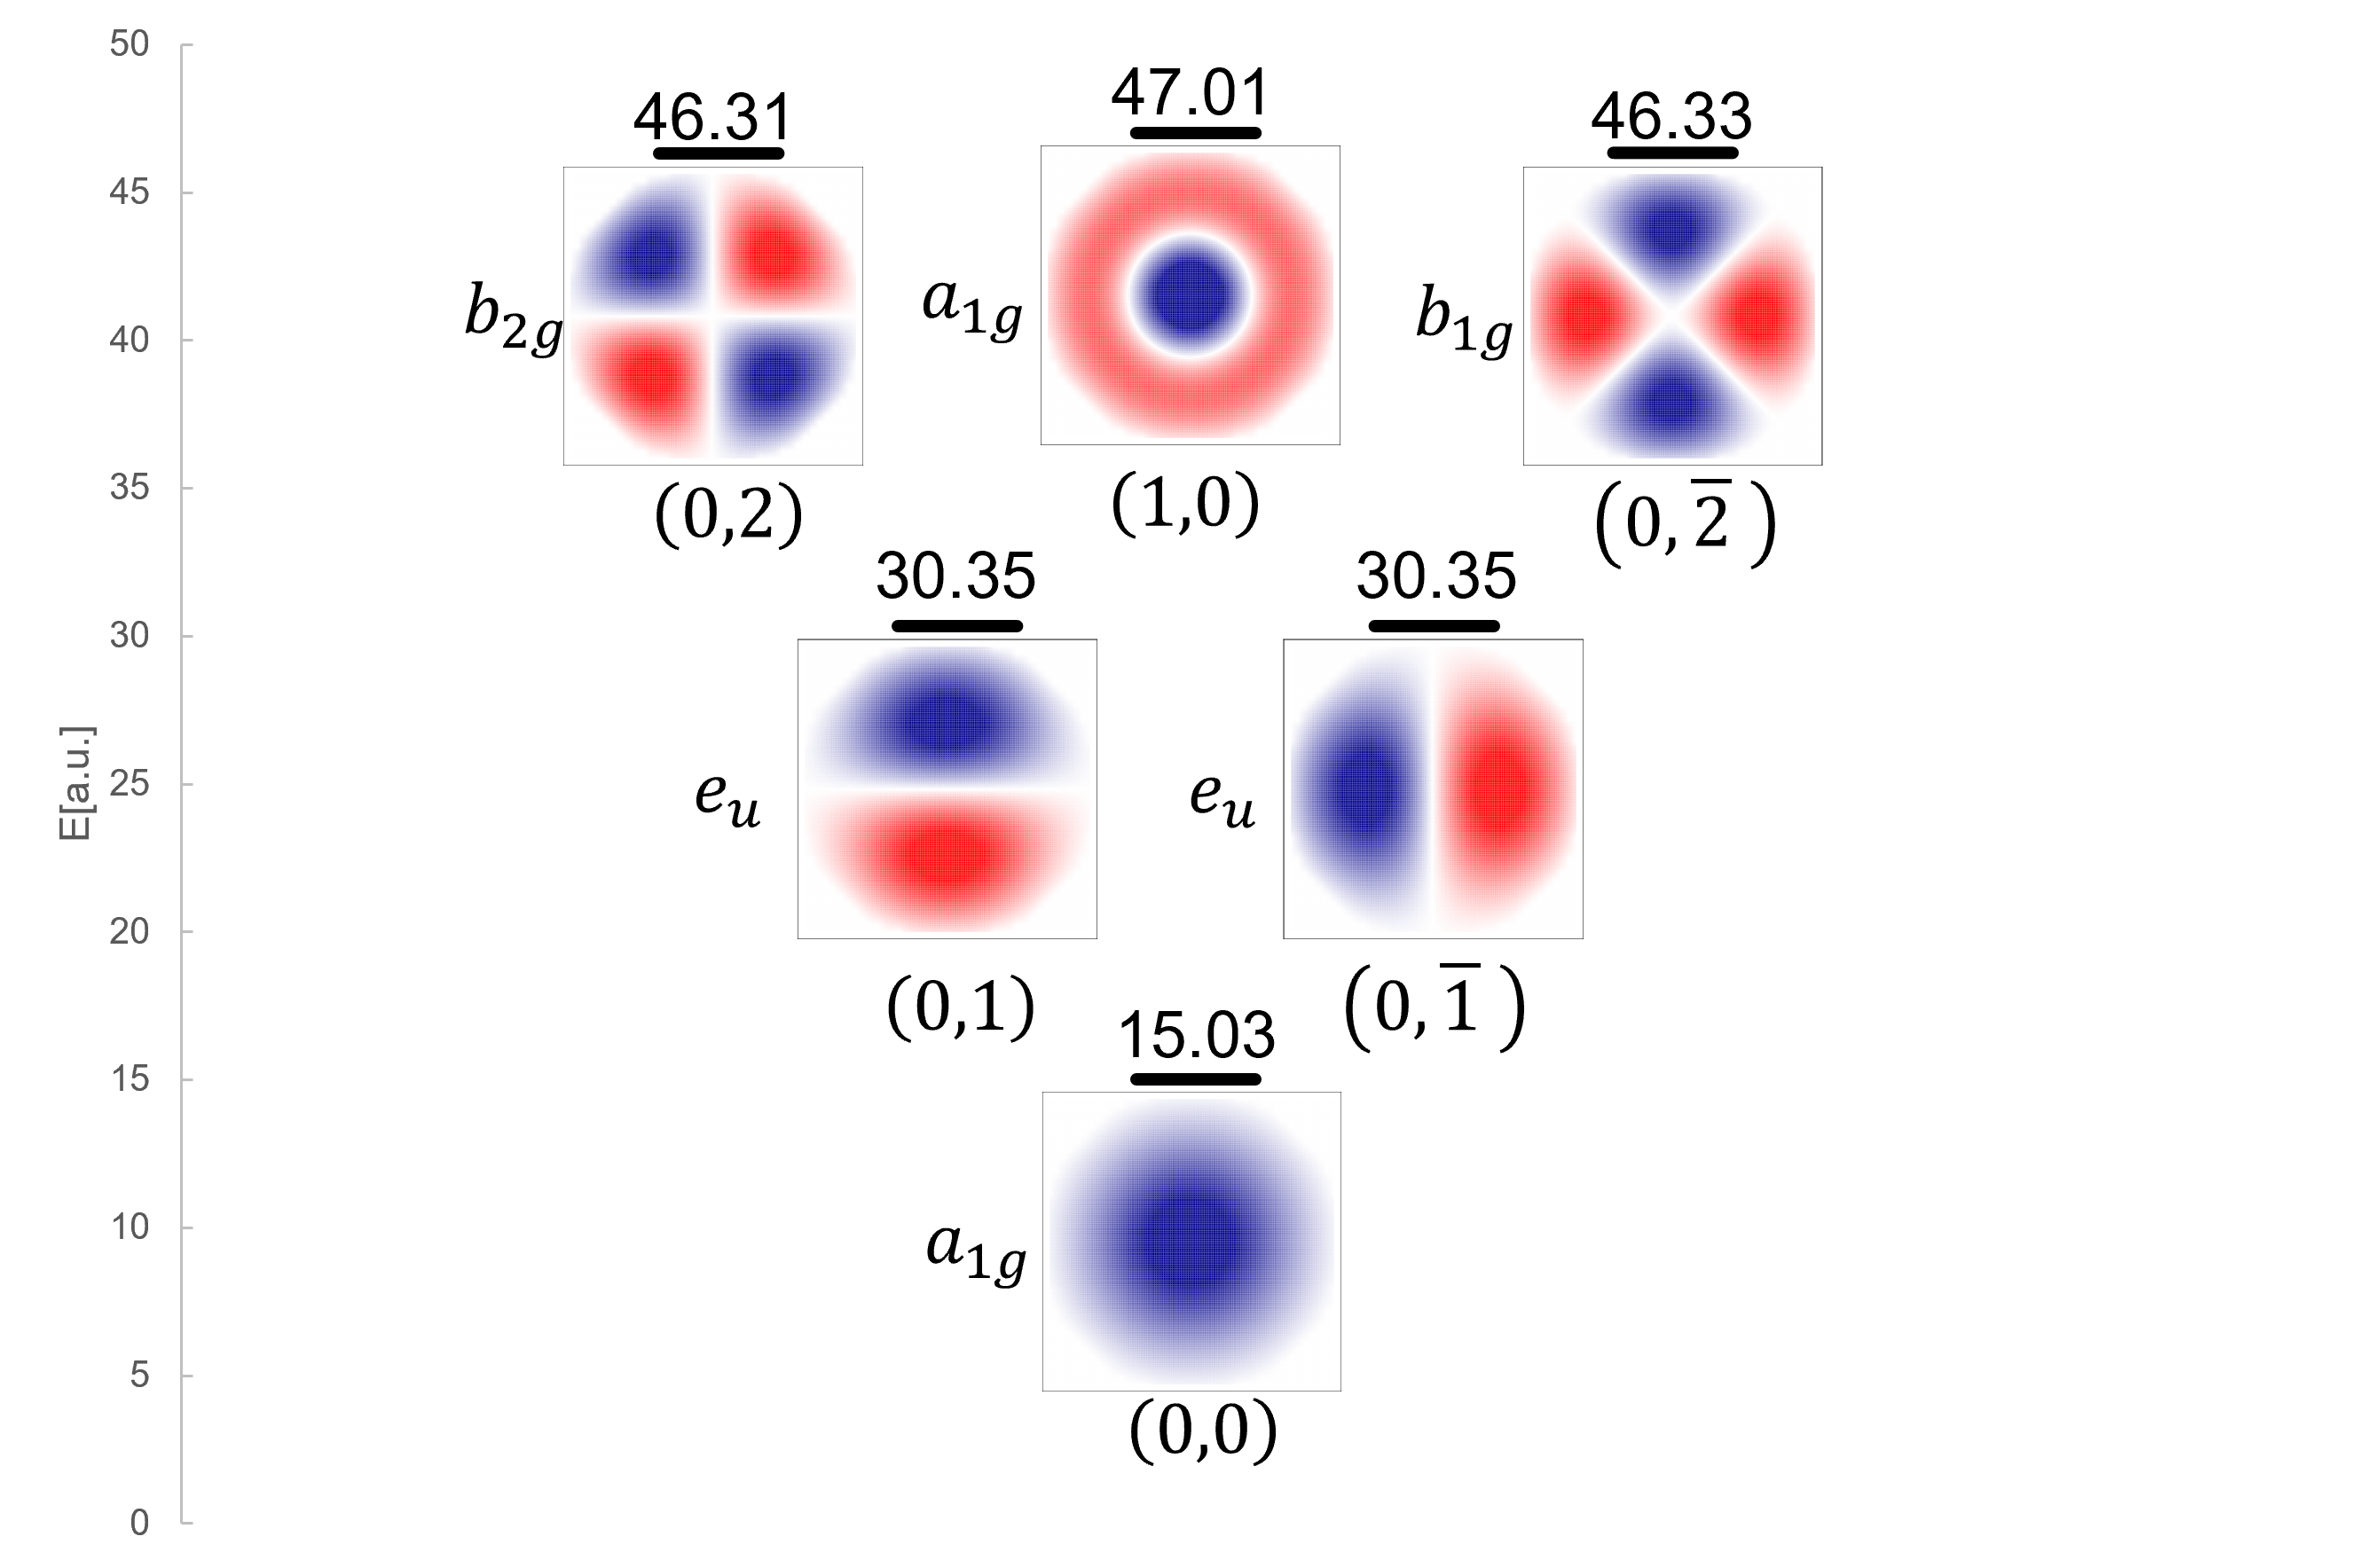
\includegraphics[width=1.30\linewidth]{images/ハイブリッド準位図.png} \\
            \scriptsize 図5.4:ハイブリッド数値解準位図
          \end{center}
          

          \column{0.32\textwidth}
          \begin{center}
            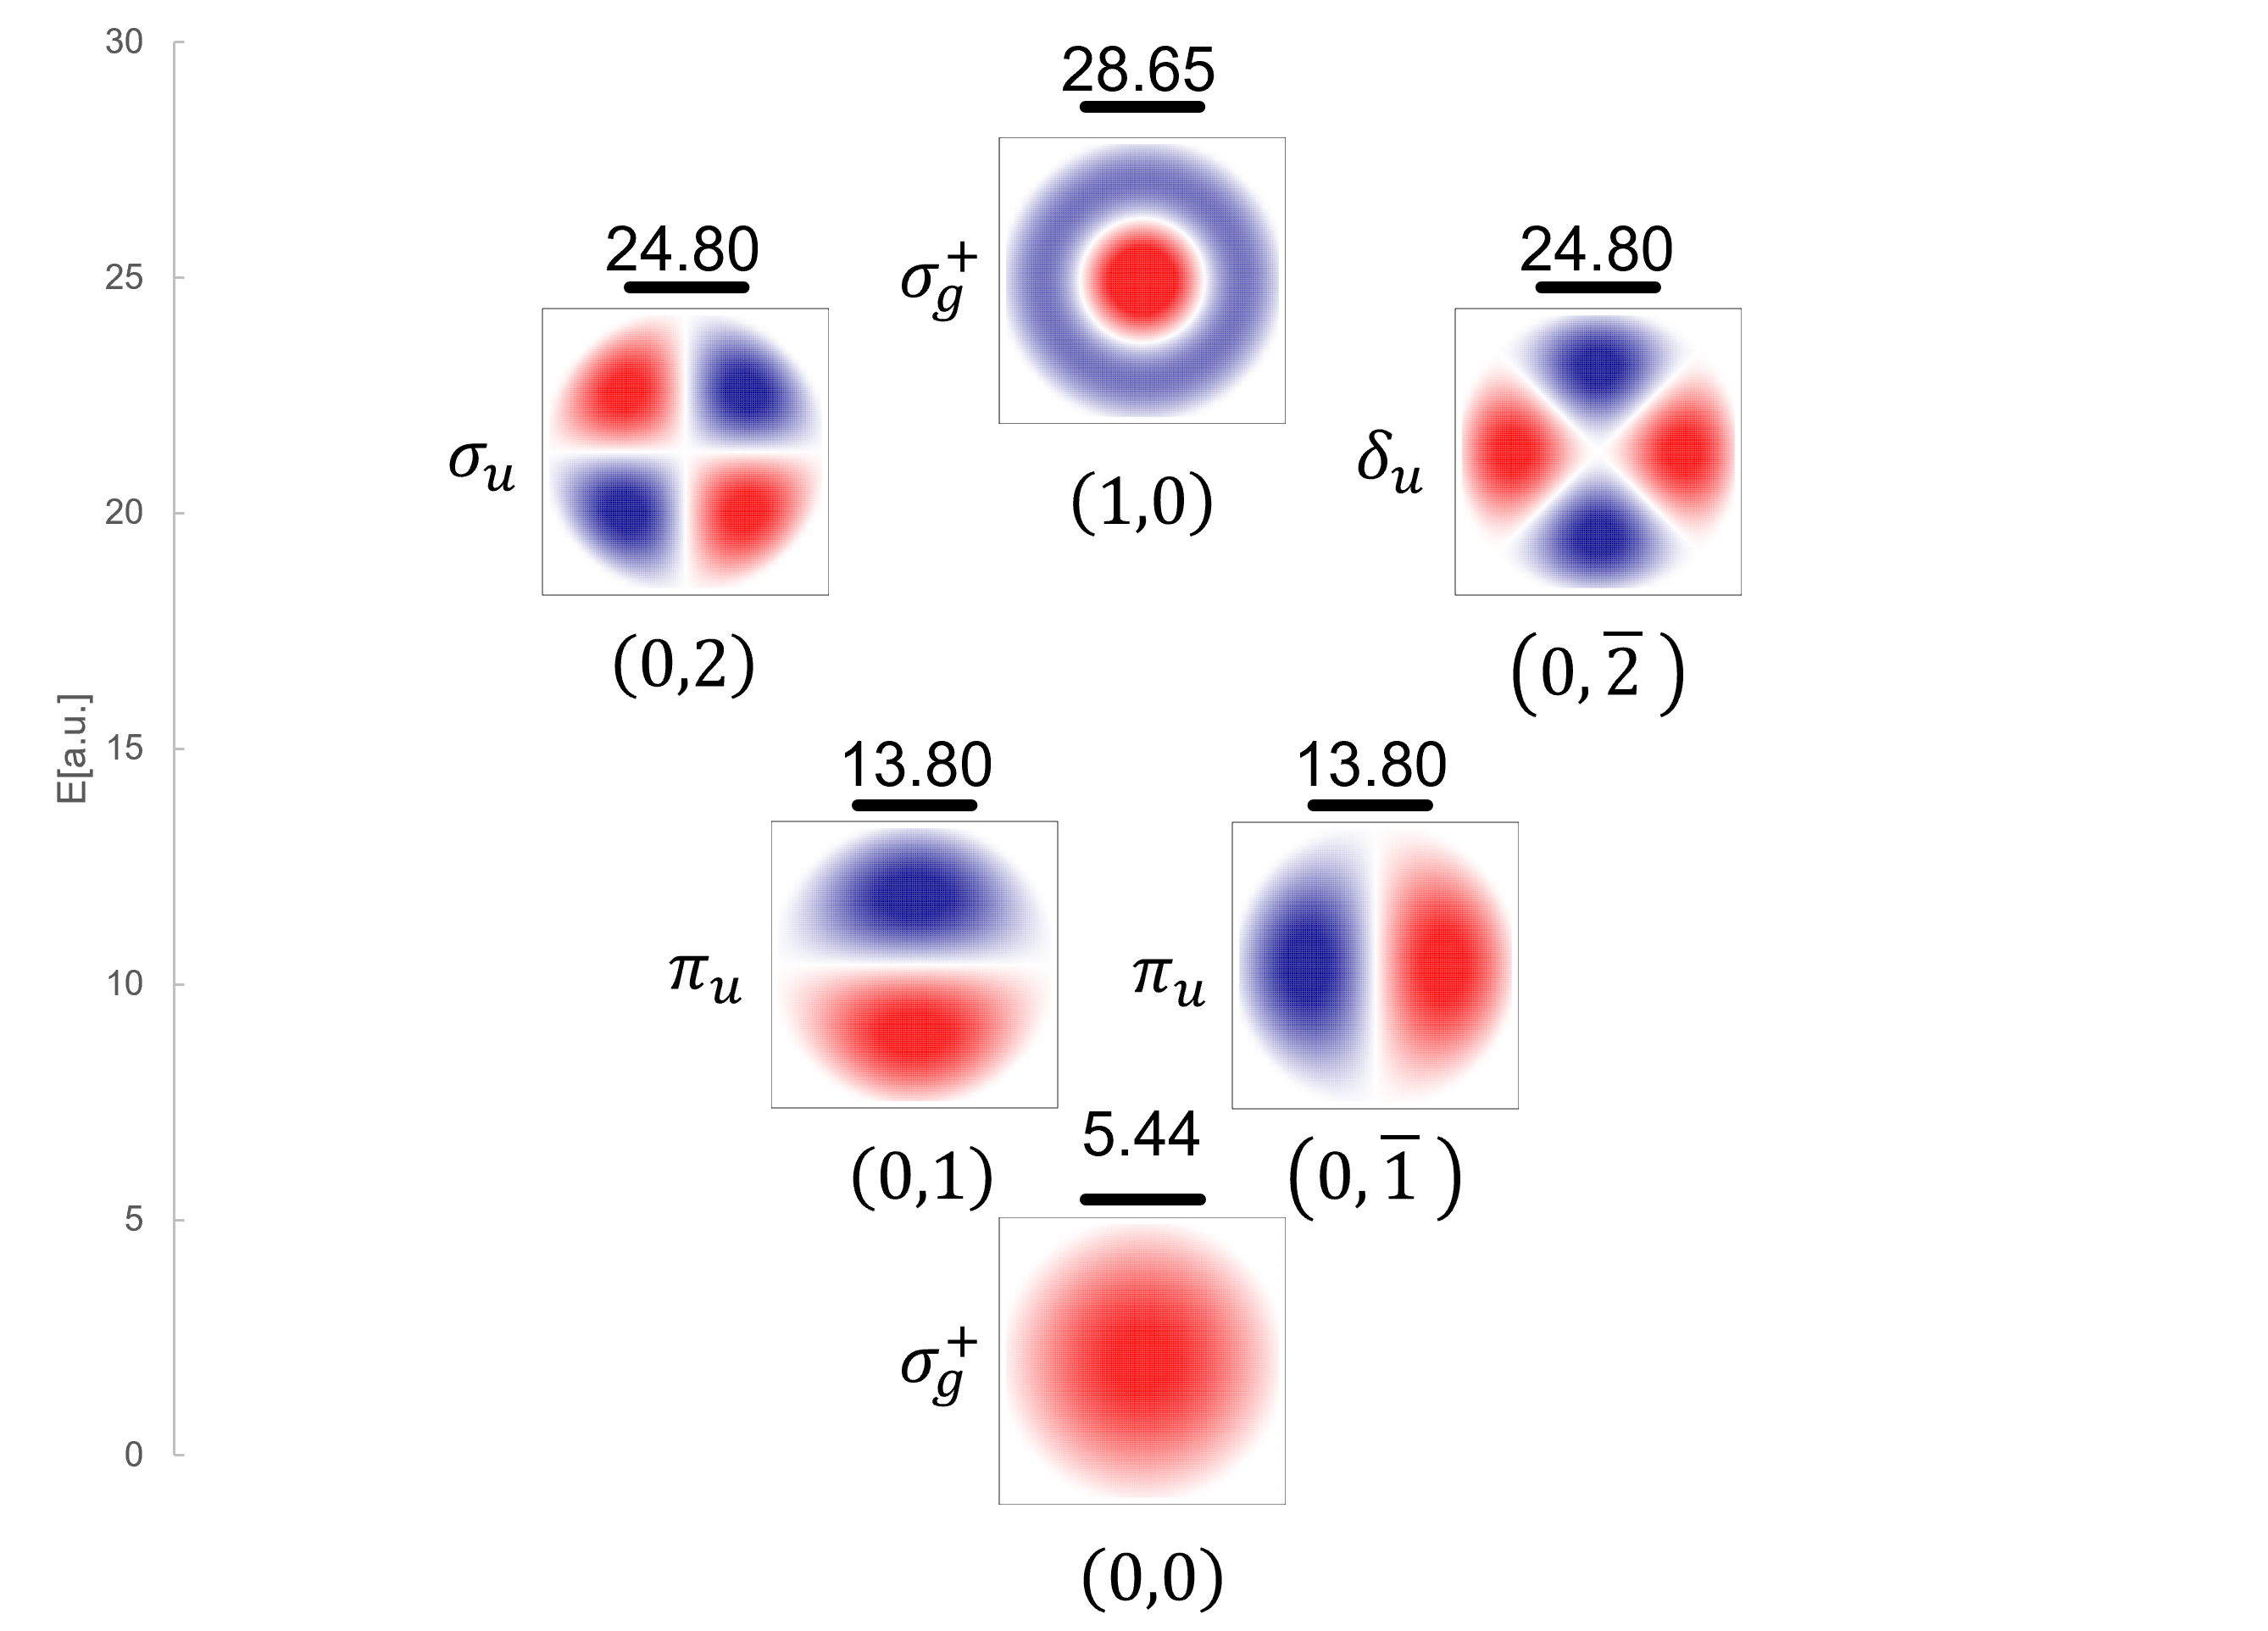
\includegraphics[width=1.30\linewidth]{images/円筒準位図.png} \\
            \scriptsize 図5.5:円筒解析解準位図
          \end{center}


          \end{columns}
          

    
    \end{frame}
    
    \begin{frame}{}
      \textbf{演習④\quad 計算結果の解析}
    
          閉じ込め強度 $\omega$ を変化させて以下を比較せよ:
          \begin{itemize}
            \item 調和ポテンシャルの解析解
            \item ハイブリッドポテンシャルの数値解
          \end{itemize}
          
          \begin{center}
            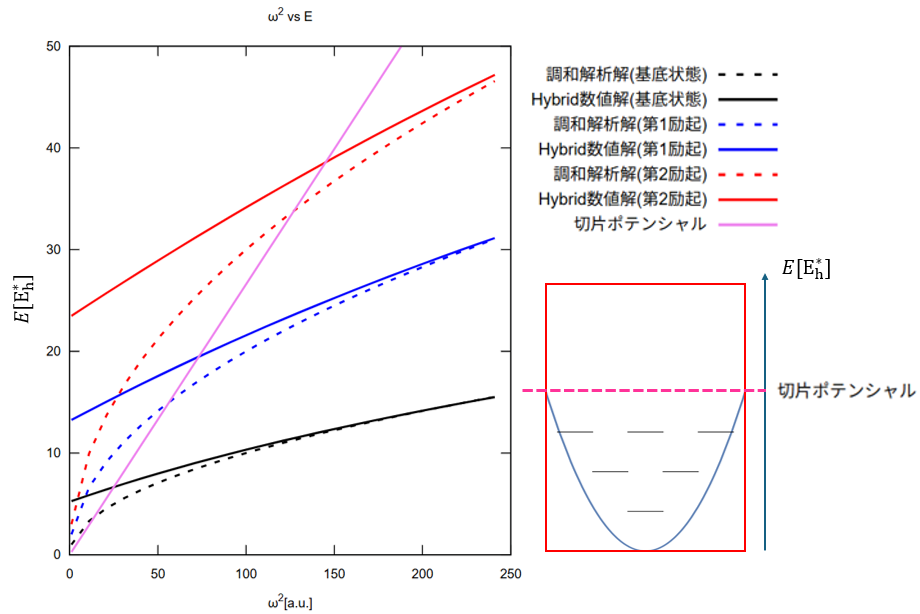
\includegraphics[width=0.92\linewidth]{images/閉じ込め強度変化改.png} \\
            図5.6:エネルギーの閉じ込め強度依存性
          \end{center}
    
    \end{frame}
    
    \begin{frame}{課題}
    
        \begin{enumerate}
          \item 演習①の結果をまとめる.
          \item 演習②の結果をまとめる.
          \item 以上の演習結果をもとに,以下を含む PDF を作成して提出:
          \begin{itemize}
            \item 演習③ の結果と考察
            \item 演習④ の結果と考察
            \item 感想
          \end{itemize}
        \end{enumerate}
        
        \textbf{提出先}:\\
        \url{https://waseda.app.box.com/f/accd8d004f054cfc96d3fa131416db19} \\
        
        \textbf{質問等はこちらまで}:\\
        \texttt{m2@qms.cache.waseda.ac.jp}
    
    \end{frame}
  

  
\end{document}